%%%%%%%%%%%%%%%%%%%%%%%%%%%%%%%%%%%%%%%%%


\documentclass[24pt,a4paper]{article}
%\documentclass[tikz, border=2mm]{standalone}
\usepackage{tikz}
\usetikzlibrary{matrix,calc}
\usepackage{graphicx}

\usepackage[utf8]{inputenc} % Required for inputting international characters
\usepackage[T1]{fontenc} % Output font encoding for international characters

\usepackage{mathpazo} % Palatino font
\usepackage{float}

\newcommand{\implicantsol}[3][0]{
	\draw[rounded corners=3pt, fill=#3, opacity=0.3] ($(#2.north west)+(135:#1)$) rectangle ($(#2.south east)+(-45:#1)$);
}


%internal group
%#1 - Optional. Space between node and grouping line. Default=0
%#2 - top left node
%#3 - bottom right node
%#4 - filling color
\newcommand{\implicant}[4][0]{
	\draw[rounded corners=3pt, fill=#4, opacity=0.3] ($(#2.north west)+(135:#1)$) rectangle ($(#3.south east)+(-45:#1)$);
}

%group lateral borders
%#1 - Optional. Space between node and grouping line. Default=0
%#2 - top left node
%#3 - bottom right node
%#4 - filling color
\newcommand{\implicantcostats}[4][0]{
	\draw[rounded corners=3pt, fill=#4, opacity=0.3] ($(rf.east |- #2.north)+(90:#1)$)-| ($(#2.east)+(0:#1)$) |- ($(rf.east |- #3.south)+(-90:#1)$);
	\draw[rounded corners=3pt, fill=#4, opacity=0.3] ($(cf.west |- #2.north)+(90:#1)$) -| ($(#3.west)+(180:#1)$) |- ($(cf.west |- #3.south)+(-90:#1)$);
}

%group top-bottom borders
%#1 - Optional. Space between node and grouping line. Default=0
%#2 - top left node
%#3 - bottom right node
%#4 - filling color
\newcommand{\implicantdaltbaix}[4][0]{
	\draw[rounded corners=3pt, fill=#4, opacity=0.3] ($(cf.south -| #2.west)+(180:#1)$) |- ($(#2.south)+(-90:#1)$) -| ($(cf.south -| #3.east)+(0:#1)$);
	\draw[rounded corners=3pt, fill=#4, opacity=0.3] ($(rf.north -| #2.west)+(180:#1)$) |- ($(#3.north)+(90:#1)$) -| ($(rf.north -| #3.east)+(0:#1)$);
}

%group corners
%#1 - Optional. Space between node and grouping line. Default=0
%#2 - filling color
\newcommand{\implicantcantons}[2][0]{
	\draw[rounded corners=3pt, opacity=.3] ($(rf.east |- 0.south)+(-90:#1)$) -| ($(0.east |- cf.south)+(0:#1)$);
	\draw[rounded corners=3pt, opacity=.3] ($(rf.east |- 8.north)+(90:#1)$) -| ($(8.east |- rf.north)+(0:#1)$);
	\draw[rounded corners=3pt, opacity=.3] ($(cf.west |- 2.south)+(-90:#1)$) -| ($(2.west |- cf.south)+(180:#1)$);
	\draw[rounded corners=3pt, opacity=.3] ($(cf.west |- 10.north)+(90:#1)$) -| ($(10.west |- rf.north)+(180:#1)$);
	\fill[rounded corners=3pt, fill=#2, opacity=.3] ($(rf.east |- 0.south)+(-90:#1)$) -|  ($(0.east |- cf.south)+(0:#1)$) [sharp corners] ($(rf.east |- 0.south)+(-90:#1)$) |-  ($(0.east |- cf.south)+(0:#1)$) ;
	\fill[rounded corners=3pt, fill=#2, opacity=.3] ($(rf.east |- 8.north)+(90:#1)$) -| ($(8.east |- rf.north)+(0:#1)$) [sharp corners] ($(rf.east |- 8.north)+(90:#1)$) |- ($(8.east |- rf.north)+(0:#1)$) ;
	\fill[rounded corners=3pt, fill=#2, opacity=.3] ($(cf.west |- 2.south)+(-90:#1)$) -| ($(2.west |- cf.south)+(180:#1)$) [sharp corners]($(cf.west |- 2.south)+(-90:#1)$) |- ($(2.west |- cf.south)+(180:#1)$) ;
	\fill[rounded corners=3pt, fill=#2, opacity=.3] ($(cf.west |- 10.north)+(90:#1)$) -| ($(10.west |- rf.north)+(180:#1)$) [sharp corners] ($(cf.west |- 10.north)+(90:#1)$) |- ($(10.west |- rf.north)+(180:#1)$) ;
}

%Empty Karnaugh map 4x4
\newenvironment{Karnaugh}%
{
	\begin{tikzpicture}[baseline=(current bounding box.north),scale=0.8]
		\draw (0,0) grid (4,4);
		\draw (0,4) -- node [pos=0.7,above right,anchor=south west] {AB} node [pos=0.7,below left,anchor=north east] {Cs2Cs1} ++(135:1);
		%
		\matrix (mapa) [matrix of nodes,
		column sep={0.8cm,between origins},
		row sep={0.8cm,between origins},
		every node/.style={minimum size=0.3mm},
		anchor=8.center,
		ampersand replacement=\&] at (0.5,0.5)
		{
			\& |(c00)| 00         \& |(c01)| 01         \& |(c11)| 11         \& |(c10)| 10         \& |(cf)| \phantom{00} \\
			|(r00)| 00             \& |(0)|  \phantom{0} \& |(1)|  \phantom{0} \& |(3)|  \phantom{0} \& |(2)|  \phantom{0} \&                     \\
			|(r01)| 01             \& |(4)|  \phantom{0} \& |(5)|  \phantom{0} \& |(7)|  \phantom{0} \& |(6)|  \phantom{0} \&                     \\
			|(r11)| 11             \& |(12)| \phantom{0} \& |(13)| \phantom{0} \& |(15)| \phantom{0} \& |(14)| \phantom{0} \&                     \\
			|(r10)| 10             \& |(8)|  \phantom{0} \& |(9)|  \phantom{0} \& |(11)| \phantom{0} \& |(10)| \phantom{0} \&                     \\
			|(rf) | \phantom{00}   \&                    \&                    \&                    \&                    \&                     \\
		};
	}%
	{
	\end{tikzpicture}
}

%Empty Karnaugh map 2x4
\newenvironment{Karnaughvuit}%
{
	\begin{tikzpicture}[baseline=(current bounding box.north),scale=0.8]
		\draw (0,0) grid (4,2);
		\draw (0,2) -- node [pos=0.7,above right,anchor=south west] {Cs1/Cs0} node [pos=0.7,below left,anchor=north east] {Cs2} ++(135:1);
		%
		
		\matrix (mapa) [matrix of nodes,
		column sep={0.8cm,between origins},
		row sep={0.8cm,between origins},
		every node/.style={minimum size=0.9mm},
		anchor=4.center,
		ampersand replacement=\&] at (0.5,0.5)
		{
			\& |(c00)| 00         \& |(c01)| 01         \& |(c11)| 11         \& |(c10)| 10         \& |(cf)| \phantom{00} \\
			|(r00)| 0             \& |(0)|  \phantom{0} \& |(1)|  \phantom{0} \& |(3)|  \phantom{0} \& |(2)|  \phantom{0} \&                     \\
			|(r01)| 1             \& |(4)|  \phantom{0} \& |(5)|  \phantom{0} \& |(7)|  \phantom{0} \& |(6)|  \phantom{0} \&                     \\
			|(rf) | \phantom{00}  \&                    \&                    \&                    \&                    \&                     \\
		};
	}%
	{
	\end{tikzpicture}
}



\newenvironment{Karnaughvuity}%
{
	\begin{tikzpicture}[baseline=(current bounding box.north),scale=0.8]
		\draw (0,0) grid (4,2);
		\draw (0,2) -- node [pos=0.7,above right,anchor=south west] {Cs2/Cs1} node [pos=0.7,below left,anchor=north east] {B} ++(135:1);
		%
		
		\matrix (mapa) [matrix of nodes,
		column sep={0.8cm,between origins},
		row sep={0.8cm,between origins},
		every node/.style={minimum size=0.9mm},
		anchor=4.center,
		ampersand replacement=\&] at (0.5,0.5)
		{
			\& |(c00)| 00         \& |(c01)| 01         \& |(c11)| 11         \& |(c10)| 10         \& |(cf)| \phantom{00} \\
			|(r00)| 0             \& |(0)|  \phantom{0} \& |(1)|  \phantom{0} \& |(3)|  \phantom{0} \& |(2)|  \phantom{0} \&                     \\
			|(r01)| 1             \& |(4)|  \phantom{0} \& |(5)|  \phantom{0} \& |(7)|  \phantom{0} \& |(6)|  \phantom{0} \&                     \\
			|(rf) | \phantom{00}  \&                    \&                    \&                    \&                    \&                     \\
		};
	}%
	{
	\end{tikzpicture}
}



%Defines 8 or 16 values (0,1,X)
\newcommand{\contingut}[1]{%
	\foreach \x [count=\xi from 0]  in {#1}
	\path (\xi) node {\x};
}

%Places 1 in listed positions
\newcommand{\minterms}[1]{%
	\foreach \x in {#1}
	\path (\x) node {A};
}

%Places 0 in listed positions
\newcommand{\maxterms}[1]{%
	\foreach \x in {#1}
	\path (\x) node {0};
}

\newcommand{\aorb}[1]{%
	\foreach \x in {#1}
	\path (\x) node {AorB};
}

\newcommand{\ab}[1]{%
	\foreach \x in {#1}
	\path (\x) node {AB};
}

\newcommand{\bprime}[1]{%
	\foreach \x in {#1}
	\path (\x) node {B'};
}

\newcommand{\one}[1]{%
	\foreach \x in {#1}
	\path (\x) node {1};
}

%Places X in listed positions
\newcommand{\indeterminats}[1]{%
	\foreach \x in {#1}
	\path (\x) node {X};
}

\begin{document}

%----------------------------------------------------------------------------------------
%	TITLE PAGE
%----------------------------------------------------------------------------------------

\begin{titlepage} % Suppresses displaying the page number on the title page and the subsequent page counts as page 1
	\newcommand{\HRule}{\rule{\linewidth}{0.5mm}} % Defines a new 
	
	\textsc{\LARGE CSE306 Lab Report}\\[1.5cm] % Main heading such as the name of your university/college
	
	\textsc{\Large Offline 1}\\[0.5cm] % Major heading such as course name
	
	\textsc{\Large Group - 03}\\[0.5cm] % Major heading such as course name

	
	%------------------------------------------------
	%	Title
	%------------------------------------------------
	
	\HRule\\[0.4cm]
	
	{\huge\bfseries 4-bit ALU Simulation}\\[0.4cm] % Title of your document
	
	\HRule\\[1.5cm]
	
	%------------------------------------------------
	%	Author(s)
	%------------------------------------------------
	
	\begin{minipage}{0.4\textwidth}
		\begin{flushleft}
			\large
			\textit{Group Members}\\
			\textsc{1705093} \\
			\textsc{1705098} \\
			\textsc{1705103} \\
			\textsc{1705110} \\
			\textsc{1705119} \\
			
		\end{flushleft}
	\end{minipage}

	
	
	\vfill\vfill\vfill % Position the date 3/4 down the remaining page
	
	{\large\today} % Date, change the \today to a set date if you want to be precise
	

	 

	\vfill % Push the date up 1/4 of the remaining page
	
\end{titlepage}

%--------------------2nd page-----------------------------------------------

\newpage


\section{Introduction}
\Large
An arithmetic logical unit (ALU) is a digital circuit used to perform arithmetic and logic operations. It represents the fundamental building block of the central processing unit (CPU) of a computer.\newline


The purpose of the ALU is to perform mathematical operations such as addition, subtraction, multiplication and division. Additionally, the ALU processes basic logical operations like AND/OR calculations.\newline


Unless otherwise stated, we assume that the inputs A and B are signed, two’s complement number when they are presented to the input of the ALU. The operations performed by an ALU are controlled by a set of operation-select inputs.Logical operations take place on the bits that comprise a value (known as bitwise operations), while arithmetic operations treat inputs and outputs as two’s complement integers. Errors must be detected by the ALU.If an addition results in overflow or a multiplication results in a value that cannot be shortened to 4 bits, the Overflow flag must be enabled. 


% 3rd page

\newpage

\section{Problem Specification}

\Large
We are going to design an ALU for the following specifications


\begin{table}[H]
	
	\caption{Design Spec for Group-03} \label{tab:sometab} 
	\break
	\centering
	\begin{tabular}{|l|l|l|l|} \hline
		
		Cs2 & Cs1 & Cs0/Cin & Function             \\ \hline
		0   & 0   & 0       & Subtract with borrow \\ \hline
		0   & 0   & 1       & Subtract             \\ \hline
		0   & 1   & 0       & Transfer A           \\ \hline
		0   & 1   & 1       & Increment A          \\ \hline
		1   & 0   & x       & OR                   \\ \hline
		1   & 1   & x       & AND                  \\ \hline
	    
	\end{tabular}
	
\end{table}

\section{Truth table and K-Maps}

\begin{table}[H]
	
	\caption{Truth Table for $X_i, Y_i, Z_i$} \label{tab:sometab} 
	\break
	\centering
	\begin{tabular}{|l|l|l|l|l|l|} \hline
		
		Cs2 & Cs1 & Cs0  & $X_i$     & $Y_i$ & $Z_i$         \\ \hline
		0   & 0   & 0    &   A       &   B'   & 0          \\ \hline
		0   & 0   & 1    &   A       &   B'   & 1         \\ \hline
		0   & 1   & 0    &   A       &   0    &	0		\\ \hline
		0   & 1   & 1    &   A       &   0    & 1  		\\ \hline
		1   & 0   & x    & $A\vee B$ &   0    & 0      		\\ \hline
		1   & 1   & x    &   AB      &   0    & 0      		\\ \hline
		
	\end{tabular}
	
\end{table}

\subsection{K-Maps for $X_i$}
\Large
\begin{Karnaugh}
	\maxterms{0,1,4,5,8,12,13,14}
	\one{2,3,6,7,9,10,11,15}
	\implicant{3}{2} {yellow}
	\implicant{11}{10} {yellow}
	\implicant{3}{2} {blue}
	\implicant{7}{6} {blue}
	\implicant{15}{11} {red}
	\implicant{3}{7} {red}
	\implicant{9}{11} {green}
\end{Karnaugh}

\newpage
So the final equation for $X_i$ ,\newline
	$X_i$ \\ 
    $  = AB + Cs_2Cs_1'B + Cs_1'A + Cs_2'A $\\    
	$  = A(B+Cs_2'+Cs_1') + BCs_2Cs_1'$\\

\subsection{K-Map for $Y_i$}
\begin{Karnaughvuity}
	\one{0}
	\maxterms{1,2,3,4,5,6,7}
		
\end{Karnaughvuity}
\begin{center}
	$Y = Cs_2'Cs_1'B'$
\end{center}


\subsection{K-Map for $Z_i$}
\begin{Karnaughvuit}
	\one{1,3}
	\maxterms{0,2,4,5,6,7}
	\implicant{1}{3}{green}
	
\end{Karnaughvuit}
\begin{center}
	$Z = Cs_2'Cs_0$
\end{center}

\newpage

\section{Block Diagram}

\begin{figure}[H]
	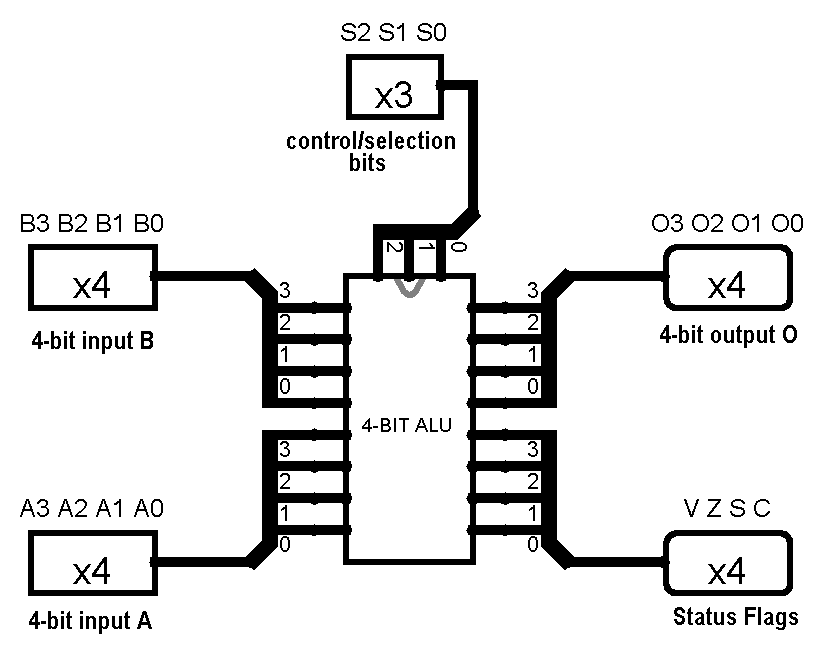
\includegraphics[width=16cm , height=18cm]{block.png}
	\caption{Block Diagram of a 4 bit ALU}
\end{figure}

\section{Circuit Diagram}

\begin{figure}[H]
	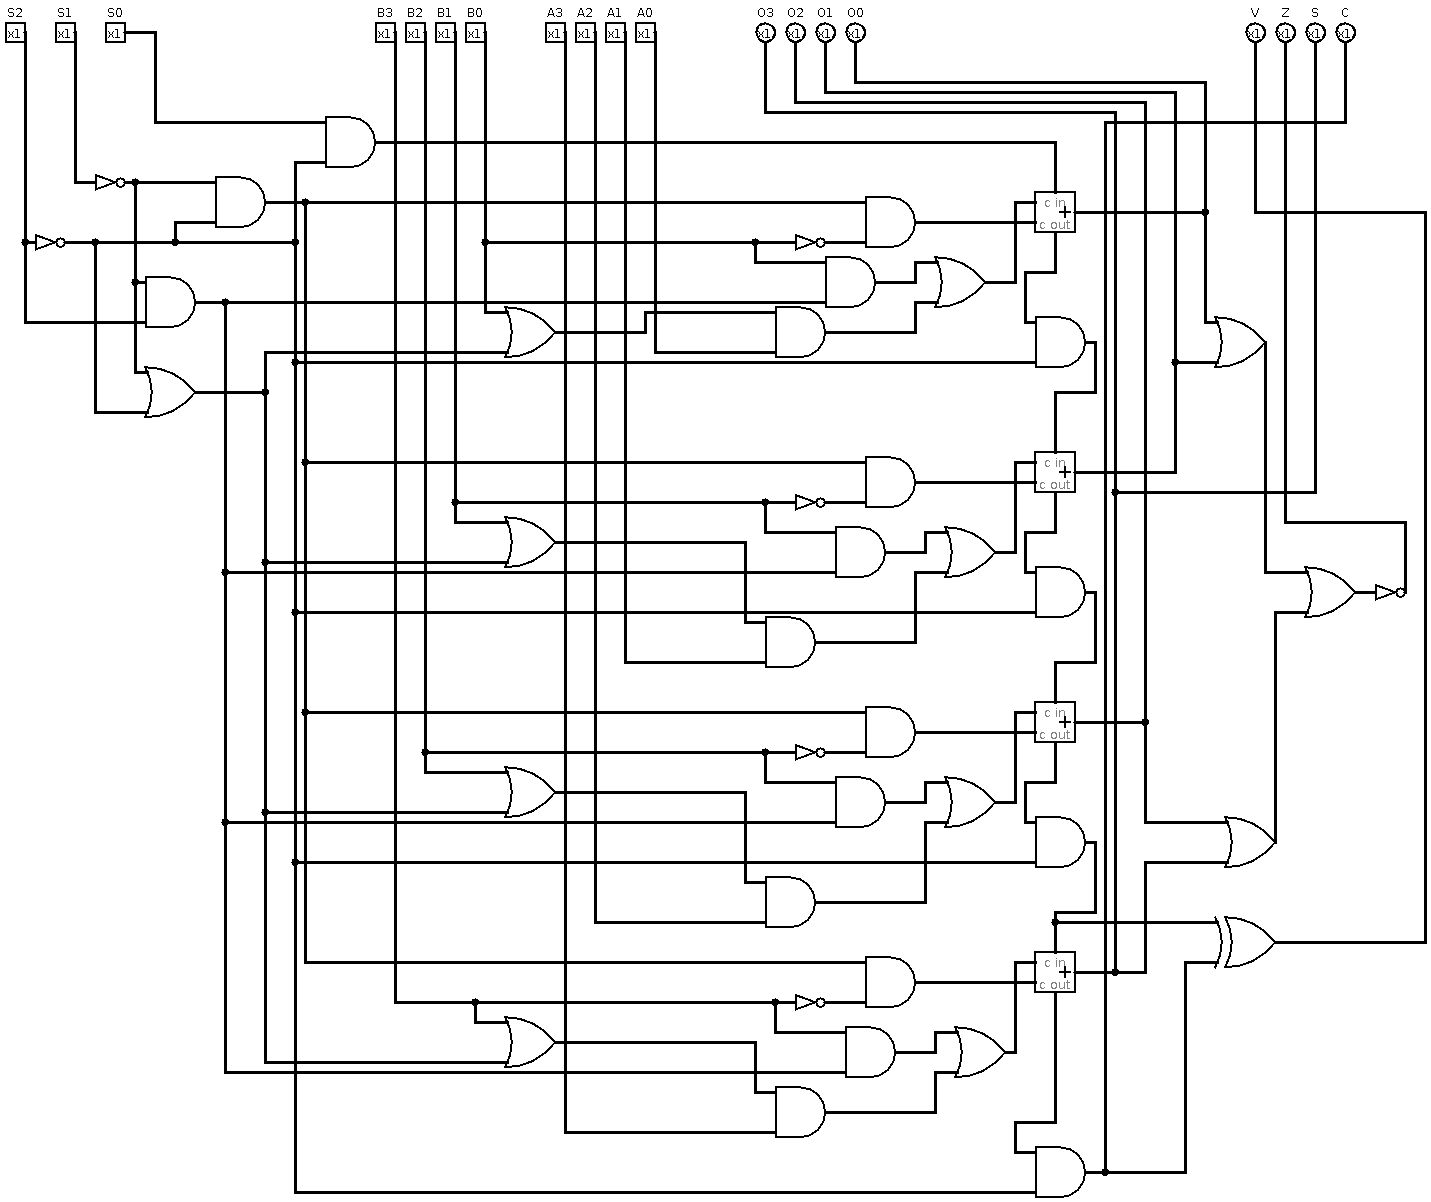
\includegraphics[width=15cm , height=18cm]{ckt.png}
	\caption{Circuit Diagram of A 4 Bit ALU}
\end{figure}


\section{ICs used with count as a chart}

\begin{table}[H]
	\centering
	\begin{tabular}{|l|l|l|l|l|l|l|} \hline
		Gate & Base Count & Count/Adder & Total & IC   & IC Count \\ \hline
		AND  & 3          & 4           & 19    & 7408 & 5  \\ \hline
		OR   & 4          & 2           & 12    & 7432 & 3  \\ \hline
		NOT  & 3          & 1           & 7     & 7404 & 2   \\ \hline
		XOR  & 1          & -           & 1     & 7486 & 1  \\ \hline
	\end{tabular}
	\caption{Gates and IC chart}
\end{table}

\section{Simulation Platform}
\Large
Logisim-2.7.10
\section{Discussion}
\Large
We tried to make our implementation as efficient as possible. To achieve this at first we 
applied gate level minimization using K-Maps. From the resulting SOPs of the K-Maps, we applied 
some basic Boolean algebra to minimize the number of gates further.

When implementing our design, we identified parts of the circuitry that were common for each of the 
4 bits. Then we reused the common parts to avoid inefficiency due to redundancy. 

Even though we designed the circuit using basic gates, we tried to minimize the number of ICs that would
be needed if this circuit were to be implemented in lab using the 7400 series ICs. We did this by keeping
the following idea in mind while designing and implementing : "When a new operation is needed try to use 
empty slots on existing ICs instead of using a gate that would require a new IC"

While implementing we tried to place the ICs in a systematic manner so that the logic being implemented by
the gates is readily obvious to anyone looking at the circuit diagram.

Finally, we created a block diagram version of our ALU design and tested our design with various inputs. This level
of abstraction made it easier to verify inputs/outputs without having to think about the underlying design each time.



\end{document}
